\chapter{Errors in Dataset Similarity in Datasets and Images}
Step 2 og our scheme




\section{Labelling errors}
\noindent Labels are crucial because they serve as the foundation for training and evaluating machine learning models, particularly in supervised learning
\begin{itemize}
    \item Ground truth: the labels that the AI model should learn to predict or approximate
\end{itemize}

\subsubsection{Labels in databases for AI}
\begin{itemize}
    \item Model training: key in semi and supervised learning
\end{itemize}
\begin{figure}[H]
    \centering
    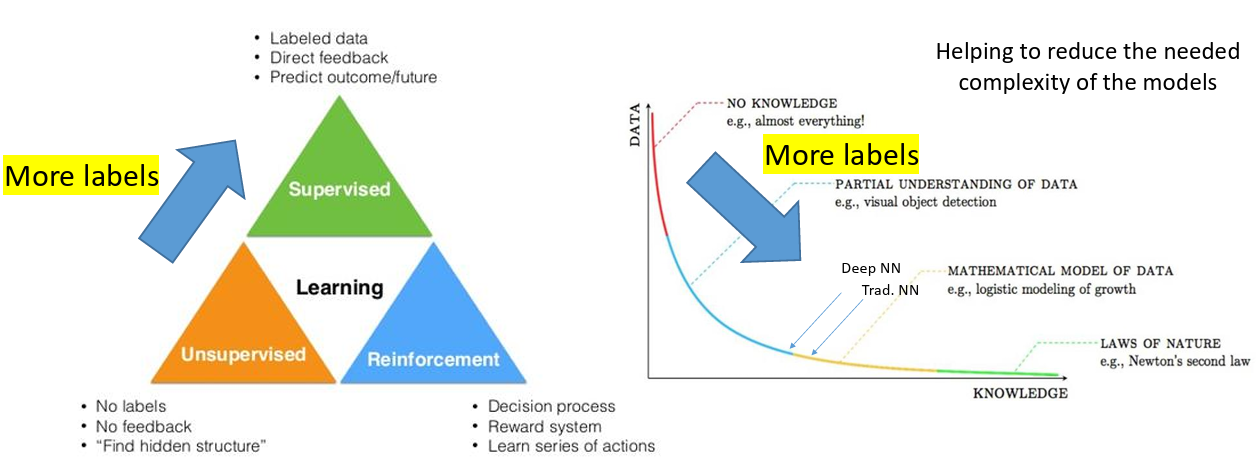
\includegraphics[width=0.8\linewidth]{09-10/images/labels.png}
\end{figure}

MANCA UN PEZZO

\subsubsection{Label Errors in Dataset}
\noindent Some examples of labeling errors are from the previous lessons
\begin{itemize}
    \item Sample is correct, but the label is wrong (it's a dog but AI says it's a cat)
    \item The sample is misleading or incomplete (Data Leakage)
\end{itemize}

\noindent \textbf{Human supervisors are the typical sources of labels for our datasets}
\begin{itemize}
    \item Direct supervisor errors
    \item Data interchange/automatic conversion errors (un bodybuilder non è grasso)
\end{itemize}

\subsubsection{Basic checks for labelling errors}
\begin{itemize}
    \item Same input vectors 
    \begin{itemize}
        \item With same labels 
        \item With opposite labels (training problems!)
    \end{itemize}
    \item What to check in the training and validation database even it is not easy with large DB 
\end{itemize}


\subsection{Supervisor errors}


\subsection{Changes in time}


\subsection{Automated Checks}


\section{Similarity }

\subsection{in datasets }

\subsection{in images}

\section{Main points}